% LaTeX Document for Android class @ THM
% \documentstyle[11pt]{article}
\documentclass[11pt,a4paper]{article}
\usepackage[ngerman]{babel}
\usepackage[utf8]{inputenc}
\usepackage{graphicx}
\usepackage{hyperref}
%\renewcommand{\ttdefault}{cmss}

\usepackage{lmodern}
\renewcommand{\familydefault}{\sfdefault}

%\newcommand{\changefont}[3]{
%\changefont{cmss}{m}{n} \changefont{cmss}{m}{sl} \changefont{cmss}{bx}{n} \selectfont}


% Default margins are too wide all the way around. I reset them here
\setlength{\topmargin}{-.5in}
\setlength{\textheight}{9in}
\setlength{\oddsidemargin}{.125in}
\setlength{\textwidth}{6.25in}
\begin{document}
\title{Memory - Dokumentation}
\author{A - Team\\Technische Hochschule Mittelhessen}
\renewcommand{\today}{11. September 2009}
\maketitle

\tableofcontents

\section {Prolog}
Die Gruppe A besteht aus Markus Kretsch, Frank Kevin Zey, Florian Thomas und Hagen Lauer.

\subsection{Anforderungen}

Muss
\begin{itemize}
\item Memory-Spielfeld mit sinnvoller Größe (z.B. 8x8 Karten/Felder) für 2 bis 6 Spieler.
\item Jeder Spieler bekommt einen Namen, der über Spielsitzungen hinweg gespeichert wird.
\item Über jeden Spieler wird eine Statistik angezeigt, wie z.B. Anzahl gewonnener \/ verlorener Spiele, oder Anzahl richtiger Treffer pro 100 Züge.
\end{itemize}
Kann
\begin{itemize}
\item Mehrspielermodus über mehrere Smartphones innerhalb eines LANs.
\item Weitere Spielkarten können z.B. von der SD-Karte nachinstalliert werden.
\end{itemize}
\subsection{Lösung / Idee}

\begin{itemize}

\item Bilder sollen mit Grid und Imageview dargestellt werden. Dabei bieten diese gute Möglichkeiten Klicks zu erkennen und entsprechend zu behandeln.
\item Für die Spieler wird eine SQLite Datenbank verwendet.
\item Wir haben gute Bibliotheken gefunden um die Daten der Spieler wie gewünscht statistisch auszuwerten und darzustellen.
\item Netzwerkspiele werden über WiFi und JavaSockets realisiert, dabei soll es einen Host und mehrere Clients pro Sitzung geben. Das Spielsystem muss also die entsprechende Flexibilität für lokale und Netzwerkspiele mitbringen.
\item Spielkarten sollen per .zip File von der SD Karte des Geräts nachladbar sein. Bilder werden in einer Datenbank gespeichert. Das Spiel lädt die Bilder für das Spielfeld aus der Datenbank.
\end{itemize}


%Type your text in free-format; lines can be as long
%or as short
%as you wish.
%      You can indent      or space out
%        your input 
%          text in 
%            any way you like to highlight the structure
%      of your manuscript and make it easier to edit.
%LaTeX fills lines and adjusts spacing between words to produce an
%aesthetically pleasing result.

%Completely blank lines in the input file break your text into
%paragraphs.
%To change the font for a single character, word, or set of words, 
%enclose the word and the font changing command within braces, 
%{\em like this}.
%A font changing command not enclosed in braces, like the change to \bf 
%bold here, keeps that change in effect until the end of the document or
%until countermanded by another font switch, like this change back to 
%\rm roman.

\section {Architektur}
Wir haben uns selbst als Ziel gesetzt, dass wir in 2 Richtungen entwickeln: Das Spiel Memory als sehr spezifische Implementierung und ein "'Framework"', das alle typischen Funktionen für ein rundenbasiertes Spiel mitbringt. So konnten wir mit entsprechenden Oberklassen (Game.java) und abgeleiteten Klassen (z.B. Memory.java) garantieren, dass am Ende beide Zweige zusammen führen.
Zum Framework gehört Game.java als Oberklasse aller implementierbaren rundenbasierten Spiele, eine Engine die im Wesentlichen Datenbankzugriffe kapselt, ein einfaches Menüsystem, das leicht konfigurier- und erweiterbar ist und einen statistischen Teil der mit der Datenbank zusammen arbeitet. Wir haben dann als Konkrete Implementierung für Memory die Klasse Memory.java von Game erben lassen und entsprechend für Memory angepasst. Ebenso wird die Netzwerkimplementierung eine von Game abgeleitete Klasse sein, natürlich noch mit einigen spezifischen Anpassungen zur Kommunikation der Geräte.

\subsection{Design}
Wie in \autoref{fig:memorydesign} zu sehen ist entsteht das Framework völlig unabhängig vom zu implementierenden Spiel.
\begin{figure}[!h]
\centering
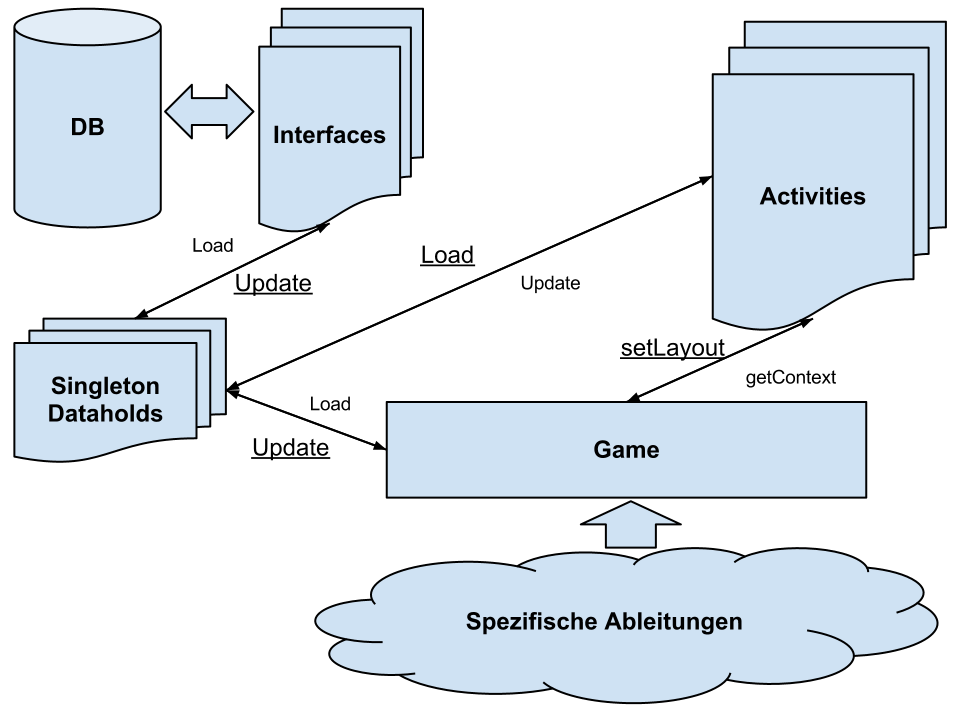
\includegraphics[scale=0.4]{pics/memorydesign.png}
\caption{Konzept}
\label{fig:memorydesign}
\end{figure}

\subsection{Engine / Datenbanken}
zeyorama
\subsection{Statistik}
crunch
\subsection{Memory}
markus
\subsection{Netzwerk}
crunch

\subsection*{Benutzerdokumentation}

Die Benutzerdokumentation wird per {\em Help} in der App bereitgestellt. 

\subsection*{Code Dokumentation}

Die Code Dokumentation ist per JavaDoc im Quelltext abgewickelt.

\end{document}
